\chapter{सांद्रता और तनुकरण}\label{ch:g10:concentration-and-dilution}

अस्पताल में मरीज़ के बिस्तर के ऊपर ड्रिप की एक थैली लटकी है। उसके लेबल पर
लिखा है ``0.9 \% सोडियम क्लोराइड'': पानी में नमक, और कुछ नहीं। फिर भी 0.9 का
आँकड़ा कोई छोटी बात नहीं। नमक बहुत कम हो, तो मरीज़ की रक्त कोशिकाएँ पानी से फूल
जाएँगी; बहुत ज़्यादा हो, तो सिकुड़ जाएँगी। किसी विलयन का वर्णन केवल उसकी सामग्री से
नहीं होता, बल्कि इससे होता है कि उसके हर आयतन में कितना \omterm{def:g6:solutions-and-solubility:solute}{विलेय} है: यही उसकी
सांद्रता है। यह अध्याय सांद्रताएँ मापता है, सटीक सांद्रता के विलयन तैयार करता है,
और उन्हें तनु करता है।

\begin{recall}
विलयन एक \omterm{def:g6:solutions-and-solubility:solute}{विलायक} और एक या अधिक घुले हुए \omterm{def:g6:solutions-and-solubility:solute}{विलेयों} से बना होता है; \omterm{def:g6:solutions-and-solubility:solubility}{विलेयता} \omterm{def:g6:solutions-and-solubility:solute}{विलेय}
का वह अधिकतम द्रव्यमान है जिसे \omterm{def:g6:solutions-and-solubility:solute}{विलायक} की दी गई मात्रा घोल सकती है
(\cref{ch:g6:solutions-and-solubility})। किसी स्पीशीज़ की मात्रा
$n = m/M$ है, \omterm{def:g10:the-mole:amount}{मोल} में (\cref{ch:g10:the-mole})।
\end{recall}

\begin{omfigure}
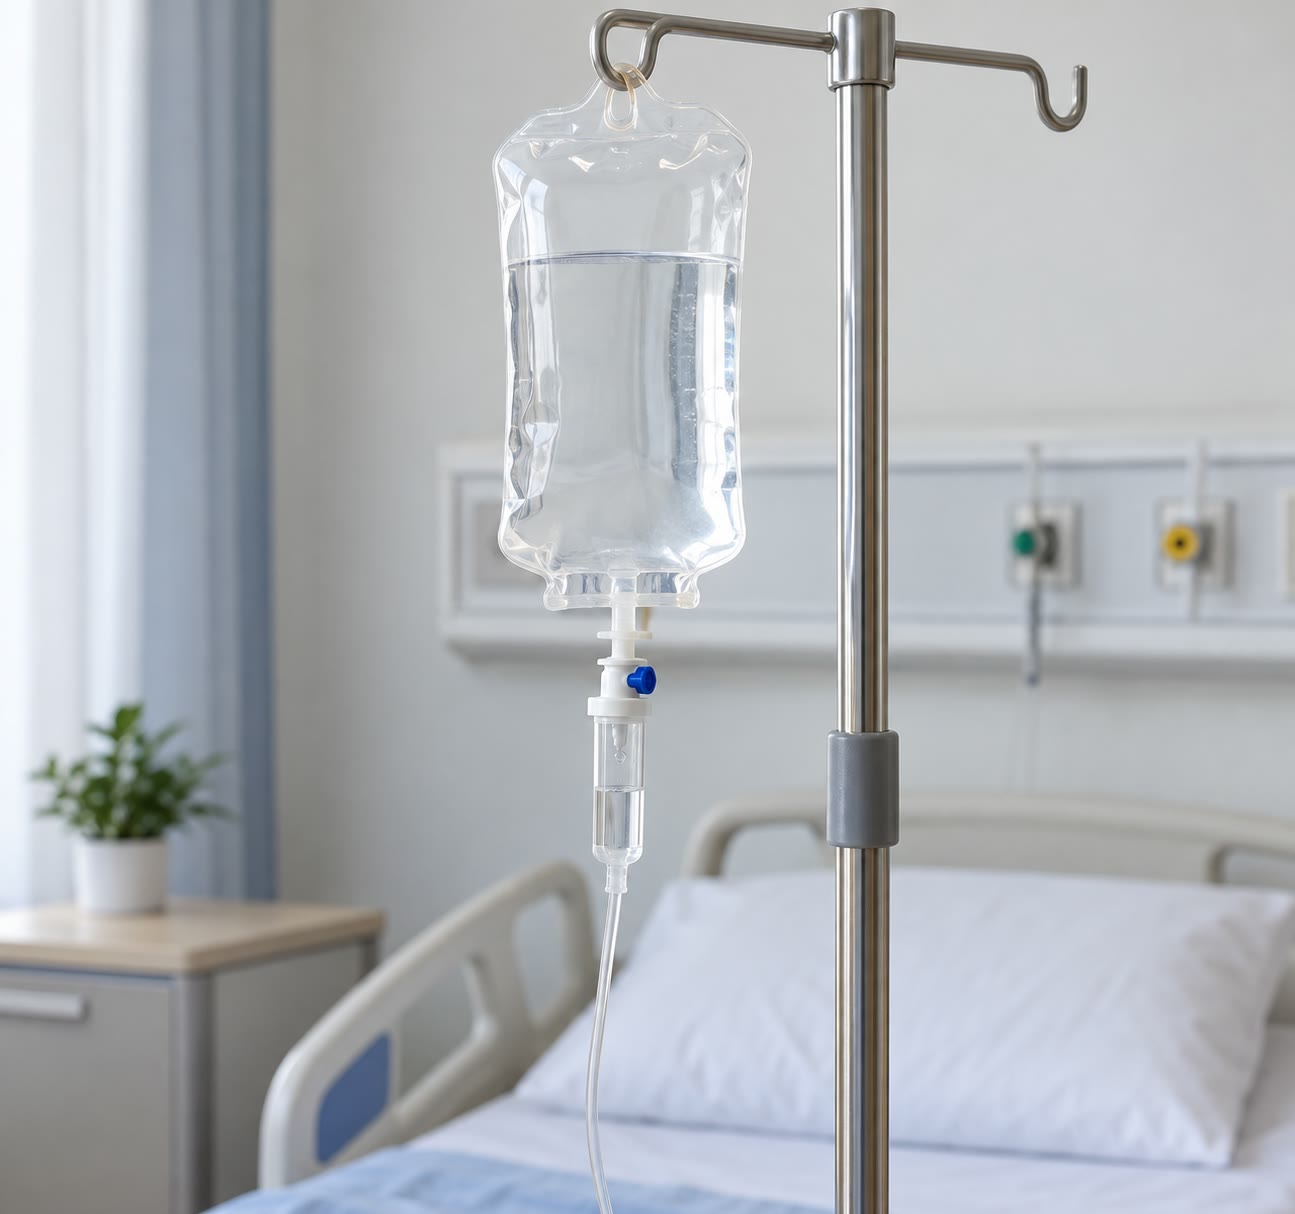
\includegraphics[width=0.42\linewidth]{images/book1/ai/g10-drip-bag.jpg}

{\small नमक के विलयन की ड्रिप-थैली: सांद्रता सही होनी चाहिए।}
\end{omfigure}

\section{द्रव्यमान सांद्रता}

\begin{definition}[द्रव्यमान सांद्रता]\label{def:g10:concentration-and-dilution:mass-concentration}
किसी विलयन में किसी \omterm{def:g6:solutions-and-solubility:solute}{विलेय} की \emph{द्रव्यमान सांद्रता}\index{द्रव्यमान सांद्रता} $C_m$
विलयन के प्रति आयतन घुले हुए \omterm{def:g6:solutions-and-solubility:solute}{विलेय} का द्रव्यमान है:
\[
  C_m = \frac{m_{\text{विलेय}}}{V_{\text{विलयन}}},
\]
ग्राम प्रति लीटर (\si{g/L}) में।
\end{definition}

\begin{example}[चीनी वाला पानी]\label{ex:g10:concentration-and-dilution:sugar}
\qty{20}{g} चीनी पानी में घोली जाती है, और विलयन का आयतन \qty{0.50}{L} तक
पूरा किया जाता है। चीनी की उसकी \omterm{def:g10:concentration-and-dilution:mass-concentration}{द्रव्यमान सांद्रता}
$C_m = \qty{20}{g} / \qty{0.50}{L} = \qty{40}{g/L}$ है। उसके किसी भी भाग की
सांद्रता यही है: उसके \qty{0.20}{L} के एक गिलास में
$\qty{40}{g/L} \times \qty{0.20}{L} = \qty{8.0}{g}$ चीनी है।
\end{example}


\begin{remark}[आयतन विलयन का है]\label{rem:g10:concentration-and-dilution:volume}
$C_m$ में आयतन पूरे विलयन का है, डाले गए पानी का नहीं: \omterm{def:g6:solutions-and-solubility:solute}{विलेय} \omterm{def:g2:mixing-and-dissolving:dissolve}{घुलने} से आयतन
थोड़ा बदल जाता है। इसीलिए विलयन को हमेशा किसी ज्ञात अंतिम आयतन तक, उसके लिए
चिह्नित फ़्लास्क में, \emph{पूरा} किया जाता है।
\end{remark}

\begin{remark}[सांद्रता विलेयता नहीं है]\label{rem:g10:concentration-and-dilution:not-solubility}
% ledger: sol:NaCl, saline:NaCl
किसी \omterm{def:g6:solutions-and-solubility:solute}{विलेय} की \omterm{def:g6:solutions-and-solubility:solubility}{विलेयता} वह \emph{अधिकतम} सांद्रता है जो वह पा सकता है; विलयन की
सांद्रता शून्य से लेकर उस तक कुछ भी हो सकती है। सोडियम
क्लोराइड \qty{25}{\celsius} पर प्रति किलोग्राम पानी लगभग \qty{360}{g} तक \omterm{def:g2:mixing-and-dissolving:dissolve}{घुलता}
है; ड्रिप-थैली में प्रति लीटर केवल \qty{9}{g} है, संतृप्ति से
बहुत दूर।
\end{remark}

\begin{remark}[लेबलों पर प्रतिशत]\label{rem:g10:concentration-and-dilution:percent}
% ledger: saline:NaCl
दवाओं और खाद्य पदार्थों के लेबलों पर पानी में घुले किसी ठोस के लिए ``0.9 \%''
का आम तौर पर अर्थ होता है \qty{100}{mL} विलयन में \qty{0.9}{g} \omterm{def:g6:solutions-and-solubility:solute}{विलेय}।
ग्राम प्रति लीटर में यह दस गुना है: ड्रिप-थैली में \qty{9.0}{g/L}
सोडियम क्लोराइड है।
\end{remark}

\section{मोलर सांद्रता}

\begin{definition}[मोलर सांद्रता]\label{def:g10:concentration-and-dilution:molar-concentration}
किसी विलयन में किसी \omterm{def:g6:solutions-and-solubility:solute}{विलेय} की \emph{मोलर सांद्रता}\index{मोलर सांद्रता} $c$
विलयन के प्रति आयतन घुले हुए \omterm{def:g6:solutions-and-solubility:solute}{विलेय} की मात्रा
है:
\[
  c = \frac{n_{\text{विलेय}}}{V_{\text{विलयन}}},
\]
\omterm{def:g10:the-mole:amount}{मोल} प्रति लीटर (\si{mol/L}) में।
\end{definition}

\begin{proposition}[एक सांद्रता से दूसरी तक]\label{prop:g10:concentration-and-dilution:link}
\omterm{def:g10:the-mole:molar-mass}{मोलर द्रव्यमान} $M$ वाले \omterm{def:g6:solutions-and-solubility:solute}{विलेय} के लिए,
\[
  C_m = c \times M .
\]
\end{proposition}

\begin{proof}
$C_m = m / V = (n \times M) / V = (n / V) \times M = c \times M$।
\end{proof}

\begin{example}[ड्रिप-थैली मोल में]\label{ex:g10:concentration-and-dilution:drip}
% ledger: saline:NaCl, saline:Na, aw:Na, aw:Cl
ड्रिप-थैली में \qty{9.0}{g/L} सोडियम क्लोराइड है, जिसका \omterm{def:g10:the-mole:molar-mass}{मोलर द्रव्यमान}
\qty{58.5}{g/mol} है। उसकी \omterm{def:g10:concentration-and-dilution:molar-concentration}{मोलर सांद्रता} है
\[
  c = \frac{C_m}{M} = \frac{\qty{9.0}{g/L}}{\qty{58.5}{g/mol}}
    = \qty{0.154}{mol/L}.
\]
निर्माता का लेबल यही आँकड़ा उलटी ओर से देता है: प्रति लीटर सोडियम \omterm{def:g9:ions:ion}{आयनों} का
एक \omterm{def:g10:the-mole:amount}{मोल} का 154 हज़ारवाँ भाग।
\end{example}

\begin{remark}[विलयन में आयन]\label{rem:g10:concentration-and-dilution:ions}
सोडियम क्लोराइड अलग-अलग \omterm{def:g9:ions:ion}{आयनों} \ce{Na+} और \ce{Cl-} के रूप में \omterm{def:g2:mixing-and-dissolving:dissolve}{घुलता} है
(\cref{ch:g9:ions}): इसलिए \qty{0.154}{mol/L} वाले सोडियम क्लोराइड विलयन में
सोडियम \omterm{def:g9:ions:ion}{आयनों} की सांद्रता \qty{0.154}{mol/L} होती है और क्लोराइड \omterm{def:g9:ions:ion}{आयनों} की भी \qty{0.154}{mol/L}
होती है। कोई आयनिक ठोस पानी में कैसे बिखरता है, यह आगे के एक अध्याय
का विषय है।
\end{remark}

\begin{omfigure}
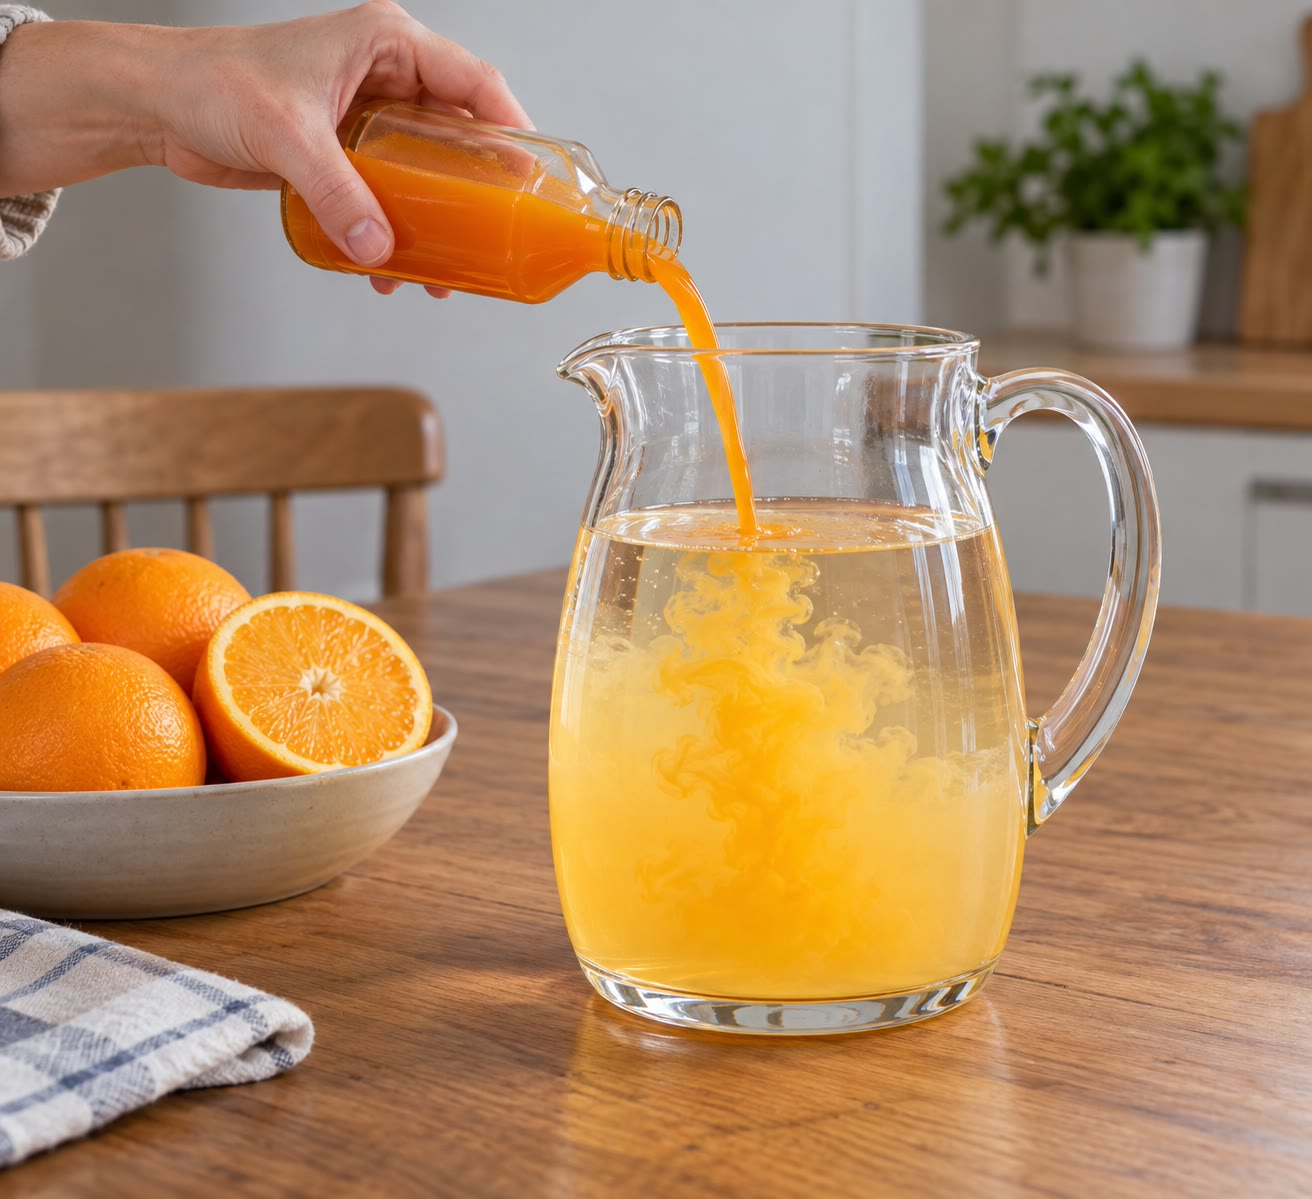
\includegraphics[width=0.45\linewidth]{images/book1/ai/g10-squash-jug.jpg}

{\small बोतल के शरबत को जग में पानी से तनु किया जाता है: पेय में फल के शरबत की
मात्रा उतनी ही है, बस बड़े आयतन में।}
\end{omfigure}

\section{घोलकर विलयन तैयार करना}

\begin{method}[ठोस घोलकर विलयन तैयार करना]\label{met:g10:concentration-and-dilution:dissolving}
किसी विलयन का आयतन $V$, \omterm{def:g10:concentration-and-dilution:molar-concentration}{मोलर सांद्रता} $c$ पर, तैयार करने के लिए:
\begin{enumerate}
  \item आवश्यक मात्रा $n = c \times V$, और तौले जाने वाले द्रव्यमान
        $m = n \times M$, की गणना कीजिए।
  \item ठोस का यह द्रव्यमान तुला पर एक छोटी प्याली में तौलिए।
  \item ठोस को कीप से आयतन $V$ वाले आयतनमितीय फ़्लास्क में डालिए; प्याली और
        कीप को आसुत जल से धोकर वह पानी भी फ़्लास्क में डालिए, ताकि कोई ठोस
        न खोए।
  \item फ़्लास्क के लगभग आधे तक आसुत जल डालिए और तब तक घुमाइए जब तक
        सारा ठोस घुल न जाए।
  \item निशान तक आसुत जल डालिए, आख़िरी बूँदें ड्रॉपर से;
        फ़्लास्क को डाट से बंद करके मिलाने के लिए कई बार उलटिए।
\end{enumerate}
\end{method}

\begin{omfigure}
\begin{tikzpicture}[font=\small, scale=1.05]
  % 1. weigh
  \pic[transform shape] at (0,0) {balance};
  \fill[black!8, draw=black!55] (-0.45,0.8) -- (0.45,0.8) -- (0.38,0.98)
    -- (-0.38,0.98) -- cycle;
  \fill[white, draw=black!40] (-0.25,0.98) .. controls (-0.1,1.15) and
    (0.1,1.15) .. (0.25,0.98) -- cycle;
  \node[align=center, anchor=north] at (0,-0.2) {1. ठोस\\ तौलिए};
  % 2. transfer through a funnel
  \pic[transform shape] at (3.2,0) {volflask={0.08}{omWater}};
  \pic[transform shape] at (3.2,3.0) {funnel};
  \draw[omProp, thick, -{Stealth}] (2.4,5.0) -- (2.85,4.65);
  \node[align=center, anchor=north] at (3.2,-0.2) {2. डालिए,\\ धोकर डालिए};
  % 3. half full, swirl
  \pic[transform shape] at (6.4,0) {volflask={0.45}{omWater}};
  \draw[omProp, thick, -{Stealth}] (5.55,0.5) arc[start angle=200,
    end angle=340, x radius=0.9, y radius=0.3];
  \node[align=center, anchor=north] at (6.4,-0.2) {3. आधा भरा:\\ घुलने तक घुमाइए};
  % 4. to the mark
  \pic[transform shape] at (9.6,0) {volflask={1}{omWater}};
  \fill[black!45] (9.43,3.6) rectangle (9.77,3.85);
  \draw[omDef, thick, <-] (9.82,2.9) -- (10.6,3.3) node[right] {निशान};
  \node[align=center, anchor=north] at (9.6,-0.2) {4. निशान तक भरिए,\\
    डाट लगाइए, मिलाइए};
\end{tikzpicture}

{\small ठोस घोलकर विलयन तैयार करना: तौलिए, डालिए, घोलिए, फिर
आयतनमितीय फ़्लास्क के निशान तक आयतन पूरा कीजिए।}
\end{omfigure}

\begin{inthelab}[निशान तक भरना]
आयतनमितीय फ़्लास्क का निशान उसकी गर्दन के चारों ओर एक छल्ला है। काँच की
सँकरी नली में पानी सपाट नहीं रुकता: उसकी सतह बीच में नीचे की ओर मुड़कर एक
नवचंद्रक बनाती है। फ़्लास्क तब भरा होता है जब नवचंद्रक का \emph{निचला भाग} निशान को
छूता है, आँख को निशान के स्तर पर रखकर देखने पर, ताकि छल्ले का आगे और पीछे का
भाग एक ही रेखा जैसा दिखे। ऊपर से या नीचे से देखने पर स्तर तब भी सही लग सकता है
जब वह सही न हो।
\end{inthelab}

\begin{omfigure}
\begin{tikzpicture}[font=\small]
  \newcommand{\neck}[2]{% x, meniscus bottom height
    \fill[omWater] (#1-0.5,0) -- (#1-0.5,{#2+0.25}) .. controls
      (#1-0.25,#2) and (#1+0.25,#2) .. (#1+0.5,{#2+0.25}) -- (#1+0.5,0) -- cycle;
    \draw[black!60, line width=0.8pt] (#1-0.5,0) -- (#1-0.5,3);
    \draw[black!60, line width=0.8pt] (#1+0.5,0) -- (#1+0.5,3);
    \draw[omDef, line width=0.9pt] (#1-0.5,1.5) -- (#1+0.5,1.5);
    \draw[black!50] (#1-0.5,{#2+0.25}) .. controls (#1-0.25,#2) and
      (#1+0.25,#2) .. (#1+0.5,{#2+0.25});}
  \newcommand{\eye}[2]{% x, y: an eye looking to the right
    \draw[black!70] (#1-0.25,#2) .. controls (#1-0.1,#2+0.18) and
      (#1+0.1,#2+0.18) .. (#1+0.2,#2) .. controls (#1+0.1,#2-0.18) and
      (#1-0.1,#2-0.18) .. (#1-0.25,#2);
    \fill[black!70] (#1+0.05,#2) circle (0.06);}
  % right
  \neck{1.5}{1.5}
  \eye{-0.4}{1.5}
  \draw[dashed, black!50] (-0.1,1.5) -- (2.4,1.5);
  \node[align=center] at (1.5,-0.55) {सही: आँख का स्तर,\\ निचला भाग निशान पर};
  % too high
  \neck{6}{1.85}
  \eye{4.1}{1.85}
  \draw[dashed, black!50] (4.4,1.85) -- (6.9,1.85);
  \node[align=center] at (6,-0.55) {बहुत ज़्यादा पानी:\\ नवचंद्रक ऊपर};
  % too low
  \neck{10.5}{0.85}
  \eye{8.6}{0.85}
  \draw[dashed, black!50] (8.9,0.85) -- (11.4,0.85);
  \node[align=center] at (10.5,-0.55) {बहुत कम पानी:\\ नवचंद्रक नीचे};
\end{tikzpicture}

{\small आयतनमितीय फ़्लास्क की गर्दन, बड़ी करके और नवचंद्रक के स्तर पर आँख रखकर
देखी गई। नीली रेखा निशान है। केवल
बाईं ओर का फ़्लास्क सही भरा है।}
\end{omfigure}

\section{तनुकरण}

\begin{definition}[तनुकरण, मूल विलयन, तनुकरण गुणांक]\label{def:g10:concentration-and-dilution:dilution}
\emph{तनुकरण}\index{तनुकरण} \omterm{def:g6:solutions-and-solubility:solute}{विलायक} मिलाकर किसी विलयन की सांद्रता घटाता है।
शुरुआत में लिया गया सांद्र विलयन
\emph{मूल विलयन}\index{मूल विलयन} है। \emph{तनुकरण
गुणांक}\index{तनुकरण गुणांक} $F$ मूल विलयन की सांद्रता और तनु
विलयन की सांद्रता का अनुपात है:
\[
  F = \frac{c_{\text{मूल}}}{c_{\text{तनु}}} .
\]
\end{definition}

\begin{proposition}[विलेय की मात्रा बनी रहती है]\label{prop:g10:concentration-and-dilution:kept}
\omterm{def:g10:concentration-and-dilution:dilution}{तनुकरण} के दौरान \omterm{def:g6:solutions-and-solubility:solute}{विलेय} की मात्रा नहीं बदलती: अगर \omterm{def:g10:concentration-and-dilution:dilution}{मूल विलयन} के आयतन
$V_0$ को, जिसकी सांद्रता $c_0$ है, आयतन $V_1$ तक पूरा किया जाए, तो तनु विलयन की
सांद्रता $c_1$ इससे मिलती है:
\[
  c_0 \times V_0 = c_1 \times V_1,
  \qquad\text{इसलिए}\qquad
  F = \frac{c_0}{c_1} = \frac{V_1}{V_0} .
\]
\omterm{def:g10:concentration-and-dilution:mass-concentration}{द्रव्यमान सांद्रताओं} के लिए भी यही सही है।
\end{proposition}

\begin{proof}
केवल \omterm{def:g6:solutions-and-solubility:solute}{विलायक} मिलाया जाता है: आयतन $V_0$ के साथ लिया गया \omterm{def:g6:solutions-and-solubility:solute}{विलेय}, मात्रा
$c_0 V_0$, पूरा का पूरा अंतिम आयतन $V_1$ में है, जहाँ वह
मात्रा $c_1 V_1$ बनाता है।
\end{proof}


\begin{method}[तनुकरण द्वारा विलयन तैयार करना]\label{met:g10:concentration-and-dilution:diluting}
किसी विलयन का आयतन $V_1$, सांद्रता $c_1$ पर, सांद्रता $c_0$ वाले
\omterm{def:g10:concentration-and-dilution:dilution}{मूल विलयन} से तैयार करने के लिए:
\begin{enumerate}
  \item लिए जाने वाले \omterm{def:g10:concentration-and-dilution:dilution}{मूल विलयन} का आयतन निकालिए,
        $V_0 = c_1 V_1 / c_0$ (यानी $V_1 / F$)।
  \item थोड़ा-सा \omterm{def:g10:concentration-and-dilution:dilution}{मूल विलयन} एक साफ़ बीकर में डालिए (बोतल से सीधे कभी पिपेट
        मत कीजिए) और निशान तक भरे आयतनमितीय पिपेट से ठीक $V_0$
        लीजिए।
  \item पिपेट को आयतन $V_1$ वाले आयतनमितीय फ़्लास्क में ख़ाली होने दीजिए।
  \item निशान तक आसुत जल डालिए, डाट लगाइए और मिलाइए।
\end{enumerate}
\end{method}

\begin{example}[दस गुना तनुकरण]\label{ex:g10:concentration-and-dilution:tenfold}
कॉपर सल्फ़ेट के एक \omterm{def:g10:concentration-and-dilution:dilution}{मूल विलयन} का $c_0 = \qty{0.10}{mol/L}$ है;
$c_1 = \qty{0.010}{mol/L}$ पर \qty{100.0}{mL} चाहिए। \omterm{def:g10:concentration-and-dilution:dilution}{तनुकरण
गुणांक} $F = 0.10 / 0.010 = 10$ है, इसलिए $V_0 = \qty{100.0}{mL} / 10 =
\qty{10.0}{mL}$: एक \qty{10.0}{mL} का पिपेट और एक \qty{100.0}{mL} का फ़्लास्क।
\end{example}

\begin{omfigure}
\begin{tikzpicture}[font=\small, scale=0.85]
  % 1. take the stock with a pipette
  \pic[transform shape] at (0,0) {beaker={0.6}{cyan!70!blue!55}};
  \pic[transform shape] at (0,0.2) {pipette={1}{cyan!70!blue!55}};
  \node[align=center, anchor=north] at (0,-0.2) {1. मूल विलयन का\\ $V_0$ पिपेट कीजिए};
  \draw[omProp, very thick, -{Stealth}] (1.3,2.6) -- (2.6,2.6);
  % 2. empty it into the flask
  \pic[transform shape] at (4,0) {volflask={0.22}{cyan!70!blue!55}};
  \pic[transform shape] at (4,2.6) {pipette={0.12}{cyan!70!blue!55}};
  \node[align=center, anchor=north] at (4,-0.2) {2. उसे फ़्लास्क में\\ ख़ाली कीजिए};
  \draw[omProp, very thick, -{Stealth}] (5.3,2.6) -- (6.6,2.6);
  % 3. water to the mark
  \pic[transform shape] at (8,0) {volflask={1}{cyan!70!blue!14}};
  \draw[omDef, thick, <-] (8.2,2.9) -- (9.1,3.4) node[right] {निशान};
  \node[align=center, anchor=north] at (8,-0.2) {3. निशान तक पानी:\\
    आयतन $V_1$};
\end{tikzpicture}

{\small \omterm{def:g10:concentration-and-dilution:dilution}{तनुकरण}: पिपेट से मापे गए \omterm{def:g10:concentration-and-dilution:dilution}{मूल विलयन} के आयतन $V_0$ को आयतनमितीय फ़्लास्क
में $V_1$ तक पूरा किया जाता है। रंग \omterm{def:g10:concentration-and-dilution:dilution}{तनुकरण गुणांक} $V_1 / V_0$ के अनुपात में
फीका पड़ता है।}
\end{omfigure}

\section{अंशांकन श्रेणी}

\begin{definition}[मानक विलयन, अंशांकन श्रेणी]\label{def:g10:concentration-and-dilution:standard}
\emph{मानक विलयन}\index{मानक विलयन} वह विलयन है जिसकी सांद्रता यथार्थ रूप से
ज्ञात हो। \emph{अंशांकन
श्रेणी}\index{अंशांकन श्रेणी} एक ही \omterm{def:g6:solutions-and-solubility:solute}{विलेय} के मानक विलयनों की एक श्रृंखला है,
बढ़ती सांद्रताओं पर, जिसे आम तौर पर एक ही \omterm{def:g10:concentration-and-dilution:dilution}{मूल विलयन} को तनु करके बनाया जाता है;
किसी अज्ञात विलयन की उससे तुलना अज्ञात की सांद्रता का अनुमान देती है।
\end{definition}

\begin{example}[नीली श्रेणी]\label{ex:g10:concentration-and-dilution:scale}
\qty{0.20}{mol/L} वाले कॉपर सल्फ़ेट के एक \omterm{def:g10:concentration-and-dilution:dilution}{मूल विलयन} से छह \omterm{def:g10:concentration-and-dilution:standard}{मानक विलयन}
0.02, 0.04, 0.06, 0.08, 0.10 और \qty{0.12}{mol/L} पर तैयार किए जाते हैं, हर
एक एक जैसी नलियों में, एक ही ऊँचाई तक भरा हुआ। अज्ञात सांद्रता वाला एक विलयन,
उसी तरह की नली में, \qty{0.06}{mol/L} वाली नली से गहरा और
\qty{0.08}{mol/L} वाली से हल्का दिखता है: उसकी सांद्रता दोनों के बीच, लगभग
\qty{0.07}{mol/L}, है।
\end{example}

\begin{omfigure}
\begin{tikzpicture}[font=\small]
  \foreach \i/\c/\p in {0/0.02/8, 1/0.04/16, 2/0.06/24, 3/0.08/32,
                        4/0.10/40, 5/0.12/48} {
    \pic at (1.2*\i,0) {testtube={0.75}{cyan!70!blue!\p}};
    \node[anchor=north] at (1.2*\i,-0.15) {\c};
  }
  \pic at (8.4,0) {testtube={0.75}{cyan!70!blue!28}};
  \node[anchor=north] at (8.4,-0.15) {?};
  \draw[black!40] (7.55,-0.6) -- (7.55,3.2);
  \node[anchor=north] at (3,-0.7) {सांद्रता (\si{mol/L})};
  \node[anchor=north] at (8.4,-0.7) {अज्ञात};
\end{tikzpicture}

{\small कॉपर सल्फ़ेट विलयनों की एक \omterm{def:g10:concentration-and-dilution:standard}{अंशांकन श्रेणी} और एक अज्ञात
विलयन। अज्ञात तीसरी और चौथी नली के बीच है।}
\end{omfigure}

\begin{safety}{\ghs[0.82cm]{GHS05}\ghs[0.82cm]{GHS07}\ghs[0.82cm]{GHS09}}
% ledger: ghs:CuSO4
कॉपर सल्फ़ेट के विलयन: निगलने पर हानिकारक, त्वचा में जलन करने वाले, आँखों के लिए
हानिकारक, जलीय जीवों के लिए अत्यंत विषैले। चश्मा और दस्ताने; इस्तेमाल हुए विलयन
उपचार के लिए इकट्ठे किए जाते हैं, कभी नाली में नहीं बहाए जाते।
\end{safety}

\begin{remark}[आँख की सीमाएँ]\label{rem:g10:concentration-and-dilution:eye}
आँख केवल ``इन दो नलियों के बीच'' कह सकती है। किसी विलयन के रंग से सांद्रता को
अधिक बारीकी से मापने के लिए रसायनज्ञ मापते हैं कि वह कितना प्रकाश अवशोषित करता है;
आगे का एक अध्याय ठीक यही करता है।
\end{remark}

\section{अभ्यास}

\begin{exercise}[$\star$]\label{exo:g10:concentration-and-dilution:1}
\qty{5.0}{g} चीनी घोलकर \qty{250}{mL} विलयन बनाया जाता है।
चीनी की \omterm{def:g10:concentration-and-dilution:mass-concentration}{द्रव्यमान सांद्रता} ग्राम प्रति लीटर में निकालिए।
\end{exercise}

\begin{exercise}[$\star$]\label{exo:g10:concentration-and-dilution:2}
\qty{200}{mL} के एक विलयन में \qty{0.050}{mol} ग्लूकोस है।
उसकी \omterm{def:g10:concentration-and-dilution:molar-concentration}{मोलर सांद्रता} निकालिए।
\end{exercise}

\begin{exercise}[$\star$]\label{exo:g10:concentration-and-dilution:3}
\qty{0.10}{mol/L} वाला \qty{100.0}{mL} विलयन तैयार करने के लिए निर्जल कॉपर सल्फ़ेट
\ce{CuSO4} का कितना द्रव्यमान तौलना होगा?
\end{exercise}

\begin{exercise}[$\star$]\label{exo:g10:concentration-and-dilution:4}
\qty{1.0}{mol/L} वाले एक \omterm{def:g10:concentration-and-dilution:dilution}{मूल विलयन} को \qty{0.050}{mol/L} तक तनु किया जाता है।
\omterm{def:g10:concentration-and-dilution:dilution}{तनुकरण गुणांक} क्या है? \qty{100.0}{mL} तनु विलयन बनाने के लिए \omterm{def:g10:concentration-and-dilution:dilution}{मूल विलयन} का
कितना आयतन चाहिए?
\end{exercise}

\begin{exercise}[$\star$]\label{exo:g10:concentration-and-dilution:5}
सोडियम क्लोराइड के एक विलयन की \omterm{def:g10:concentration-and-dilution:molar-concentration}{मोलर सांद्रता}
\qty{0.10}{mol/L} है। उसकी \omterm{def:g10:concentration-and-dilution:mass-concentration}{द्रव्यमान सांद्रता} क्या है?
\end{exercise}

\begin{exercise}[$\star\star$]\label{exo:g10:concentration-and-dilution:6}
\qty{0.020}{mol/L} वाला \qty{250.0}{mL} विलयन तैयार करने के लिए \qty{0.50}{mol/L}
वाले \omterm{def:g10:concentration-and-dilution:dilution}{मूल विलयन} का कितना आयतन लेना होगा? इस्तेमाल होने वाले काँच के दो
उपकरणों के नाम बताइए।
\end{exercise}

\begin{exercise}[$\star\star$]\label{exo:g10:concentration-and-dilution:7}
सटीक सांद्रता का विलयन अंशांकित बीकर के बजाय आयतनमितीय फ़्लास्क में क्यों बनाया
जाता है? \omterm{def:g10:concentration-and-dilution:dilution}{मूल विलयन} का आयतन मापक सिलिंडर के बजाय आयतनमितीय पिपेट से क्यों
मापा जाता है?
\end{exercise}

\begin{exercise}[$\star\star$]\label{exo:g10:concentration-and-dilution:8}
कॉपर सल्फ़ेट की \omterm{def:g10:concentration-and-dilution:standard}{अंशांकन श्रेणी} देखिए। एक दूसरा अज्ञात विलयन
\qty{0.04}{mol/L} वाली नली से हल्का पर \qty{0.02}{mol/L} वाली से गहरा है। उसकी
सांद्रता का अनुमान लगाइए। अधिक परिशुद्ध अनुमान के लिए श्रेणी को कैसे बदला जा
सकता है?
\end{exercise}

\begin{exercise}[$\star\star$]\label{exo:g10:concentration-and-dilution:9}
ड्रिप के लिए ग्लूकोस के एक विलयन में \qty{50}{g/L} ग्लूकोस
\ce{C6H12O6} है। उसकी \omterm{def:g10:concentration-and-dilution:molar-concentration}{मोलर सांद्रता} निकालिए।
\end{exercise}

\begin{exercise}[$\star\star$]\label{exo:g10:concentration-and-dilution:10}
\qty{342}{g} सुक्रोस \ce{C12H22O11} घोलकर \qty{1.00}{L} विलयन बनाकर एक
शीरा तैयार किया जाता है। उसकी \omterm{def:g10:concentration-and-dilution:molar-concentration}{मोलर सांद्रता} निकालिए। फिर उसे दस गुना तनु किया
जाता है। तनु शीरे की \qty{20}{mL} की एक चम्मच में सुक्रोस का कितना द्रव्यमान
है?
\end{exercise}

\begin{exercise}[$\star\star$]\label{exo:g10:concentration-and-dilution:11}
एक विलयन की \omterm{def:g10:concentration-and-dilution:mass-concentration}{द्रव्यमान सांद्रता} \qty{12}{g/L} है। उसकी सांद्रता क्या होगी
(क) उसका आयतन दुगना करने तक पानी मिलाने के बाद; (ख) उसके आधे पानी
का \omterm{def:g3:separating-mixtures:evaporate}{वाष्पन} होने के बाद, जबकि सारा \omterm{def:g6:solutions-and-solubility:solute}{विलेय}
घुला रहे?
\end{exercise}

\begin{exercise}[$\star\star\star$]\label{exo:g10:concentration-and-dilution:12}
\qty{0.10}{mol/L} वाले एक विलयन को दस गुना तनु किया जाता है, परिणाम को फिर दस
गुना, और एक बार और।
\begin{enumerate}
  \item अंतिम सांद्रता क्या है?
  \item 1000 गुना के एक ही \omterm{def:g10:concentration-and-dilution:dilution}{तनुकरण} के बजाय यह तीन चरणों में क्यों किया जाता है
        (काँच के उपकरणों के आवश्यक आयतनों के बारे में सोचिए)?
\end{enumerate}
\end{exercise}

\begin{exercise}[$\star\star\star$]\label{exo:g10:concentration-and-dilution:13}
\qty{11.1}{g} कैल्सियम क्लोराइड \ce{CaCl2} घोलकर
\qty{500.0}{mL} विलयन बनाया जाता है। पानी में ठोस कैल्सियम \omterm{def:g9:ions:ion}{आयनों}
\ce{Ca^2+} और क्लोराइड \omterm{def:g9:ions:ion}{आयनों} \ce{Cl-} में बिखर जाता है।
\begin{enumerate}
  \item घुले हुए कैल्सियम क्लोराइड की \omterm{def:g10:concentration-and-dilution:molar-concentration}{मोलर सांद्रता} निकालिए।
  \item विलयन में कैल्सियम \omterm{def:g9:ions:ion}{आयनों} और क्लोराइड \omterm{def:g9:ions:ion}{आयनों} की \omterm{def:g10:concentration-and-dilution:molar-concentration}{मोलर
        सांद्रताएँ} निकालिए।
\end{enumerate}
\end{exercise}

\begin{exercise}[$\star\star\star$]\label{exo:g10:concentration-and-dilution:14}
\qty{100.0}{mL} के एक आयतनमितीय फ़्लास्क की गर्दन का भीतरी व्यास
\qty{1.2}{cm} है। एक छात्र उसे इस तरह भरता है कि नवचंद्रक का निचला भाग निशान से
\qty{2}{mm} ऊपर रहता है।
\begin{enumerate}
  \item कितना अतिरिक्त पानी डाल दिया गया है (बेलन का आयतन:
        $\pi r^2 h$)?
  \item विलयन की सांद्रता कितने प्रतिशत कम है?
\end{enumerate}
\end{exercise}

\begin{exercise}[$\star\star\star$]\label{exo:g10:concentration-and-dilution:15}
\qty{0.20}{mol/L} वाले सोडियम क्लोराइड विलयन के \qty{100}{mL} को
\qty{0.10}{mol/L} वाले सोडियम क्लोराइड विलयन के \qty{300}{mL} के साथ मिलाया जाता है।
आयतनों को जुड़ने वाला मानकर \omterm{def:g6:pure-substances-and-mixtures:mixture}{मिश्रण} की सांद्रता निकालिए। क्या यह दोनों सांद्रताओं का
औसत है? समझाइए।
\end{exercise}

\section{समस्या: ड्रिप-थैली}

\begin{problem}[{सप्ताहांत समस्या --- ``0.9 \%'' लवण-विलयन की एक थैली में नमक के
सांद्र विलयन का कितना भाग जाता है?}]
\label{pb:g10:concentration-and-dilution:1}
% ledger: saline:NaCl, saline:Na, sol:NaCl, aw:Na, aw:Cl, const:NA
एक अस्पताल की फ़ार्मेसी प्रयोगशाला में सोडियम क्लोराइड का एक सांद्र जीवाणुरहित विलयन
रखा है, जिसमें \qty{200}{g/L} है (उसके लेबल पर: ``20 \%'')। उसे ड्रिप में
इस्तेमाल होने वाले ``0.9 \%'' विलयन की \qty{500}{mL} की थैलियाँ, सांद्र विलयन को
जीवाणुरहित पानी से तनु करके, तैयार करनी हैं।

\medskip
\noindent\textbf{भाग I --- 0.9 \% का अर्थ।}
\begin{enumerate}
  \item लेबल ``0.9 \%'' का अर्थ है \qty{100}{mL} विलयन में \qty{0.9}{g}
        नमक। \omterm{def:g10:concentration-and-dilution:mass-concentration}{द्रव्यमान सांद्रता} \si{g/L} में बताइए।
  \item उसे मिलीग्राम प्रति मिलीलीटर में भी व्यक्त कीजिए।
  \item \qty{500}{mL} की एक थैली में सोडियम क्लोराइड का कितना द्रव्यमान है?
  \item सोडियम क्लोराइड प्रति किलोग्राम पानी लगभग \qty{360}{g} तक \omterm{def:g2:mixing-and-dissolving:dissolve}{घुलता}
        है। क्या थैली का विलयन संतृप्ति से दूर है?
  \item एक मरीज़ को एक दिन में इस विलयन का \qty{1.0}{L} दिया जाता है। यह
        नमक का कितना द्रव्यमान है?
\end{enumerate}

\medskip
\noindent\textbf{भाग II --- \omterm{def:g10:the-mole:amount}{मोल} में।}
\begin{enumerate}[resume]
  \item सोडियम क्लोराइड का \omterm{def:g10:the-mole:molar-mass}{मोलर द्रव्यमान} निकालिए।
  \item थैली के विलयन की \omterm{def:g10:concentration-and-dilution:molar-concentration}{मोलर सांद्रता} निकालिए।
  \item एक थैली में सोडियम क्लोराइड की कितनी मात्रा है?
  \item थैली में सोडियम \omterm{def:g9:ions:ion}{आयनों} और क्लोराइड \omterm{def:g9:ions:ion}{आयनों} की \omterm{def:g10:concentration-and-dilution:molar-concentration}{मोलर सांद्रताएँ}
        क्या हैं?
  \item एक थैली में कितने सोडियम \omterm{def:g9:ions:ion}{आयन} हैं?
\end{enumerate}

\medskip
\noindent\textbf{भाग III --- सांद्र विलयन से।}
\begin{enumerate}[resume]
  \item सांद्र विलयन और थैली के विलयन के बीच \omterm{def:g10:concentration-and-dilution:dilution}{तनुकरण गुणांक}
        निकालिए।
  \item एक थैली के लिए सोडियम क्लोराइड का कितना द्रव्यमान सांद्र विलयन से आना
        चाहिए? लिए जाने वाले सांद्र विलयन का आयतन
        निकालिए।
  \item \omterm{def:g10:concentration-and-dilution:dilution}{तनुकरण गुणांक} से इस आयतन की जाँच कीजिए।
  \item सांद्र विलयन की \omterm{def:g10:concentration-and-dilution:molar-concentration}{मोलर सांद्रता} निकालिए, और
        जाँचिए कि $c_0 V_0 = c_1 V_1$।
  \item तब लगभग कितना जीवाणुरहित पानी मिलाया जाता है (आयतनों को
        जुड़ने वाला मानिए)?
\end{enumerate}

\medskip
\noindent\textbf{भाग IV --- काँच के उपकरण और यथार्थता।}
\begin{enumerate}[resume]
  \item इस आयतन का कोई आयतनमितीय पिपेट नहीं होता। मिलीलीटर के दसवें भाग तक
        अंशांकित कौन-सा काँच का उपकरण इसे दे
        सकता है?
  \item यथार्थ होने के लिए अंतिम आयतन किस पात्र में पूरा किया
        जाना चाहिए?
  \item अगर सही आयतन के बजाय \qty{23.0}{mL} ले लिया जाए, तो थैली की \omterm{def:g10:concentration-and-dilution:mass-concentration}{द्रव्यमान
        सांद्रता} क्या होगी? वह कितने प्रतिशत ग़लत
        होगी?
  \item अंतिम उत्तर बताइए: \qty{500}{mL} की एक थैली में सांद्र विलयन का कितना
        आयतन जाता है?
\end{enumerate}
\end{problem}
